\subsection{The Method Comment}\label{sec:MethodComment}
The documentation comment for a method\index{method} (the \bsq{method} comment) describes its usage and its function within the class\index{class}, together with its parameters, the return value, and any exception it may throw.

%------------------------------------------------------------------------------

\subsubsection{The Comment Text}
It should be documented when the method's\index{method} actual behavior differs from what one would expect based on its name – refer to page \pageref{princ:NamingConventions:NamesAsContract}, and to chapter \tqfullvref{sec:TheNamingDictionary:Verbs}. Also any side effects must be documented here, including the modification of an argument; refer to chapter \tqfullvref{sec:MutableTypesForArguments} for more details onm this topic.

The comment text for an overriding method\index{method} can be replaced by the Javadoc\index{javadoc} tag \bdq{\{\nameref{sec:TagInheritDoc}\}}\index{inheritDoc@"@inheritDoc}. It is possible to add additional text to that inherited from the overridden method\index{method}. In fact, the tag \bdq{\{\nameref{sec:TagInheritDoc}\}}\index{inheritDoc@"@inheritDoc} copies the full method comment, including the additional tags for parameters, return values and exceptions.

The documentation comment for a non-final method\index{method} of a class\\footnote{Basically, these are non-static, public or protected methods in non-final classes.} has to provide detailed information when and how it has to be overridden. One information is whether the overriding method must call the super implementation, and under which circumstances. Usually you should avoid the requirement for calling the super implementation from an overriding method\index{method}, but that is not always appropriate or possible, therefore it is all the more important to document this. Refer to chapter \tqfullvref{sec:NonFinalMethods} about some more details regarding this topic. 

A comment for the case that calling the super implementation is needed may look like this:
\keeplisting{5}
\begin{lstlisting}[language=Comment]
*  …
*
*  @implSpec   Call this implementation before or after your code, to make
*      sure that the initialisations provided here are performed.
*
*  …
\end{lstlisting}

For more details on this refer to chapter \tqfullvref{sec:ExtendingClassesOverridingMethods}.

Usually, the documentation comment for a method\index{method} does not reveal details about a method's\index{method} implementation, but in case of empty \bdq{place holder methods}\index{method} or mount points, a sentence like below does not harm;
\keeplisting{2}
\begin{lstlisting}[language=Comment]
*  …
*  @implNote   This implementation does nothing.
*  …
\end{lstlisting}

If such a placeholder method\index{method} has a dummy or default return value, there has to be an appropriate \bdq{\nameref{sec:TagReturn}}\index{return@"@return} tag, specifying that value:
\keeplisting{3}
\begin{lstlisting}[language=Comment]
*  …
*  @implNote   This implementation does nothing.
*
*  @return Always <the default value>.
\end{lstlisting}

The tags \bdq{\nameref{sec:TagImplSpec}}\index{implSpec@"@implSpec} and \bdq{\nameref{sec:TagImplNote}}\index{implNote@"@implNote} are custom tags. Chapter \tqfullvref{sec:CustomTagsForJavaDoc} covers this topic in detail.

%------------------------------------------------------------------------------

\subsubsection{The Parameters}
For each method\index{method} parameter a \bdq{\nameref{sec:TagParam}}\index{param@"@param} tag must be added that describes the parameter in detail (if not already described in the main text of the method comment; in that case, a short sentence should be sufficient). The description has to cover the function of the parameter, its value range, and whether the parameter can be \lstinline|null|. Usually, \lstinline|null| is assumed to be an invalid argument value per default, so it has to be mentioned in the respective comment if it is allowed.

It is not enough to only give the type of the parameter in the comment; in fact, this is obsolete as it can be easily taken from the method's signature.

%------------------------------------------------------------------------------

\subsubsection{The Return Value}\label{sec:ReturnValue}
If the method\index{method} has a return value (it is not of type \lstinline|void|), a \bdq{\nameref{sec:TagReturn}}\index{return@"@return} tag needs to be added that describes the return value – even if this is done already in the comment text itself. For simple getter methods\index{method!getter method} and accessors\index{method!accessor method} you can use the \bdq{\{\nameref{sec:TagReturn} …\}}\index{return@"@return} tag as a shortcut:
\keeplisting{10}
\begin{lstlisting}
// The traditional form
/**
 *  <p>{@summary Return the current time for the default time zone as set
 *  by the operating system to the JVM.}</p>
 *  
 *  @return The current time.
 */
public final LocalTime currentTime() { return LocalTime.now(); }

// The shortcut    
/**
 *  {@return the current date.}
 */
public final LocalDate currentDate() { return LocalDate.now(); }
\end{lstlisting}
The generated output for the traditional form will look like this:
\begin{center}
	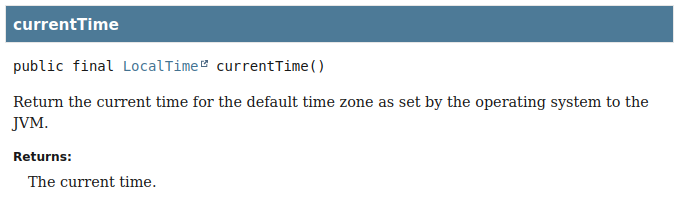
\includegraphics[scale=0.55]{comments/JavadocMethod1}
\end{center}
And the shortcut version looks like this:
\begin{center}
	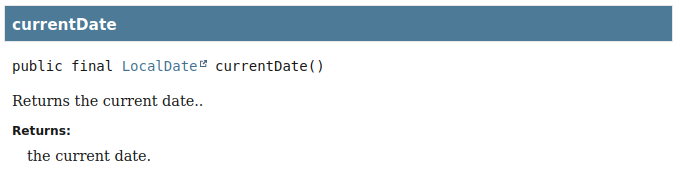
\includegraphics[scale=0.55]{comments/JavadocMethod2}
\end{center}

The only differences are the case of the letter at the beginning of the line after \bsq{\textbf{\textsf{Returns:}}} and the duplication of the full-stop for the description text. As I want to have full sentences in the documentation, I don't like the \bdq{\{\nameref{sec:TagReturn} …\}}\index{return@"@return} shortcut.

As the description of the return value should provide the possible values and their meanings, whether \lstinline|null| is a valid return value, and so on, the shortcut is usually feasible only for simple getter methods\index{method!getter method} and accessors\index{method!accessor method}, as said already above; when the text gets longer, it should be separated into the comment text and the text for the \bdq{\nameref{sec:TagReturn}}\index{return@"@return} tag. 

In particular, the description of the return value must incorporate which values indicate special or error conditions.

It is obsolete to give the type of the return value here; it can already be seen from the method's declaration.

%------------------------------------------------------------------------------

\subsubsection{The thrown Exceptions}
After the parameters and the return value follows the thrown exceptions.

Each exception that may be thrown by the method\index{method} should be declared by a  \bdq{\nameref{sec:TagThrows}}\index{throws@"@throws}; this is mandatory for each checked exception, and strongly recommended for unchecked exceptions, at least for those that the method\index{method} throws itself. 

The \bdq{\nameref{sec:TagThrows}}\index{throws@"@throws} tag lists the exception class\index{class!exception class} and describes the condition that may trigger the exception to be thrown. Refer to chapter \tqfullvref{sec:GeneralExceptionHandling} for additional details on exception handling.

%==============================================================================
% End of file!!
%==============================================================================

